\documentclass[14pt, a4paper]{article}
\usepackage{minitoc}
\usepackage[left=3.00cm, right=2.5cm, top=2.00cm, bottom=2.00cm]{geometry}
\usepackage{amsmath}
\usepackage{amssymb}
\usepackage{amsthm}
\usepackage{thmtools}
\usepackage{mathtools}
\usepackage{graphicx}
%\usepackage{algpseudocode}
%\usepackage{algorithm}
\usepackage[ruled,vlined,linesnumbered,algosection]{algorithm2e}
\usepackage{blindtext}
\usepackage{setspace}
\usepackage[utf8]{inputenc}
\usepackage[utf8]{vietnam}
\usepackage[center]{caption}
\usepackage[shortlabels]{enumitem}
\usepackage{fancyhdr} % header, footer
\usepackage{hyperref} % loại bỏ border với mục lục và công thức
\usepackage[nonumberlist, nopostdot, nogroupskip]{glossaries}
\usepackage{glossary-superragged}
\usepackage{tikz,tkz-tab}
\setglossarystyle{superraggedheaderborder}
\pagestyle{fancy}
%\usepackage[style=numeric,sortcites]{biblatex}
%\addbibresource{ref.bib}
%\usepackage[numbers]{natbib}
\usepackage{indentfirst}
\usepackage{multirow}
\usepackage[natbib,backend=biber,style=ieee, sorting=ynt]{biblatex}
\bibliography{ref.bib}

\graphicspath{{./figures/}}


\makenoidxglossaries

% Danh mục thuật ngữ

\hypersetup{
    colorlinks=false,
    pdfborder={0 0 0},
}


\fancyhf{}
\rhead{\textbf{Môn học: Một số vấn đề về đồ họa máy tính}}
\lhead{\textbf{GVHD: TS. Nguyễn Thị Bích Thủy}}
\rfoot{\thepage}
\lfoot{\textbf{Học viên thực hiện: Nguyễn Chí Thanh - 21007925}}
\renewcommand{\headrulewidth}{0.4pt}
\renewcommand{\footrulewidth}{0.4pt}


\numberwithin{equation}{section}
\numberwithin{figure}{section}

\setlength{\parindent}{0.5cm}

\setcounter{secnumdepth}{3} % Cho phép subsubsection trong report
\setcounter{tocdepth}{3} % Chèn subsubsection vào bảng mục lục

\newtheorem{dl}{Định lý}
\newtheorem{md}{Mệnh đề}
\newtheorem{bd}{Bổ đề}
\newtheorem{dn}{Định nghĩa}
\newtheorem{hq}{Hệ quả}

\numberwithin{dl}{section}
\numberwithin{md}{section}
\numberwithin{bd}{section}
\numberwithin{dn}{section}
\numberwithin{hq}{section}

\doublespacing
\AtBeginEnvironment{tabular}{\doublespacing}

\begin{document}
    \begin{titlepage}

        \newcommand{\HRule}{\rule{\linewidth}{0.5mm}} % Defines a new command for the horizontal lines, change thickness here

        \center % Center everything on the page

        %----------------------------------------------------------------------------------------
        %	HEADING SECTIONS
        %----------------------------------------------------------------------------------------
        \textsc{\LARGE Đại học Quốc Gia Hà Nội}\\[0.5cm]
        \textsc{\LARGE Trường đại học Khoa học tự nhiên}\\[0.5cm] % Name of your university/college
        \textsc{\LARGE Khoa Toán - Cơ - Tin học}\\[0.5cm]

        
\includegraphics[scale=0.2]{HUS-logo.jpg}\\[0.5cm]

        \textsc{\Large Chuyên ngành: Khoa học dữ liệu}\\[0.5cm] % Major heading such as course name


        %----------------------------------------------------------------------------------------
        %	TITLE SECTION
        %----------------------------------------------------------------------------------------

        \HRule \\[0.4cm]
        { \huge \bfseries BÀI TẬP MÔN HỌC}\\[0.4cm] % Title of your document
        \HRule \\[1.5cm]

        \textsc{\Large Môn học: Một số vấn đề về đồ họa máy tính}\\[1cm] % Minor heading such as course title


        \textsc{\Large Đề tài: Trực quan hóa văn bản và tài liệu}\\[2cm]


        %----------------------------------------------------------------------------------------
        %	AUTHOR SECTION
        %----------------------------------------------------------------------------------------
        \begin{minipage}{0.4\textwidth}
            \begin{flushleft} \large
            \emph{Giảng viên hướng dẫn:} \\
            TS. Nguyễn Thị Bích Thủy % Supervisor's Name
            \end{flushleft}
        \end{minipage}\\[0.5cm]

        \begin{minipage}{0.4\textwidth}
        \begin{flushleft} \large
        \emph{Học viên thực hiện:}\\
        Nguyễn Chí Thanh \\
        MSHV: 21007925 \\ % Your name
        Lớp: Khoa học dữ liệu - K4
        \end{flushleft}
        \end{minipage}


        % If you don't want a supervisor, uncomment the two lines below and remove the section above
        %\Large \emph{Author:}\\
        %John \textsc{Smith}\\[3cm] % Your name

        %----------------------------------------------------------------------------------------
        %	DATE SECTION
        %----------------------------------------------------------------------------------------

        % I don't want day because it is English
        % {\large \today}\\[2cm] % Date, change the \today to a set date if you want to be precise

        %----------------------------------------------------------------------------------------
        %	LOGO SECTION
        %----------------------------------------------------------------------------------------

        %\includegraphics{logo/rsz_3logo-khtn.png}\\[1cm] % Include a department/university logo - this will require the graphicx package

        %----------------------------------------------------------------------------------------

        \vfill % Fill the rest of the page with whitespace

    \end{titlepage}

    \cleardoublepage
    \pagenumbering{gobble}
    \tableofcontents
    \newpage
    \listoffigures
    \newpage
    \glsaddall 
    \renewcommand*{\glossaryname}{Danh mục các từ viết tắt}
    \renewcommand*{\acronymname}{Danh sách từ viết tắt}
    \renewcommand*{\entryname}{Viết tắt}
    \renewcommand*{\descriptionname}{Viết đầy đủ}
    \printnoidxglossary
    \cleardoublepage
    \pagenumbering{arabic}

    %\maketitle

    \newpage

    \nocite{*}

    \begin{center}
    \section*{LỜI MỞ ĐẦU}
    \end{center}
    \addcontentsline{toc}{section}{{\bf LỜI MỞ ĐẦU}\rm}

    Ta có một nguồn tài nguyên thông tin khổng lồ; từ các thư viện, đến các bộ lưu trữ email,
    đến tất cả các khía cạnh của các ứng dụng trên internet.
    Trực quan hóa là một công cụ tuyệt vời để phân tích các dữ liệu này.
    Ta có thể trực quan hóa theo nhiều dạng dữ liệu như blog, wiki, twitter feed,
    hàng tỷ từ, một tập các tờ báo hoặc một thư viện số.
    Trực quan hóa dữ liệu là một công việc phụ thuộc theo nghĩa là các công việc nào phù hợp với văn bản, tài liệu hoặc các đối tượng liên quan đến web.
    Cho dữ liệu văn bản và tài liệu, hầu hết các nhiệm vụ liên quan là tìm một từ, một cụm từ hoặc một chủ đề.
    Với dữ liệu có cấu trúc một phần, ta có thể tìm kiếm mối quan hệ giữa các từ, các cụm từ, các chủ đề hoặc giữa các tài liệu.
    Với văn bản hoặc tài liệu, nhiệm vụ chính và phổ biến nhất thường là tìm các mẫu và các điểm ngoại lai trong văn bản hoặc tài liệu.

    Đề tài này ta sẽ tập trung vào nhiệm vụ trực quan hóa dữ liệu dạng văn bản và các phương pháp tiếp cận để phân tích trực quan dữ liệu văn bản.

    \newpage

    \section{Mở đầu}

    Ta định nghĩa một tập các tài liệu là một \textit{corpus} (số nhiều là \textit{corpora}).
    Ta làm việc với các đối tượng trong corpora.
    Các đối tượng này có thể là các từ, các câu, đoạn văn, tài liệu hoặc một tập các tài liệu.
    Ta có thể xem xét cả các ảnh và video.
    Các đối tượng trên thường được xem là nguyển tử tương ứng với các nhiệm vụ, phân tích và trực quan hóa.
    Văn bản và tài liệu thường được ở dạng có cấu trúc tối thiểu và rất đa dạng các thuộc tính và metadata,
    đặc biệt khi ta tập trung vào một lĩnh vực ứng dụng cụ thể.
    Ví dụ, các tài liệu có một định dạng và thường bao gồm metadata về tài liệu (ví dụ tác giả, ngày được tạo, ngày sửa đổi, bình luận, kích thước).
    Các hệ thống truy hồi thông tin thường được dùng để truy vấn corpora, thường yêu cầu tính toán độ phù hợp của tài liệu ứng với một truy vấn.
    Nhiệm vụ này yêu cầu tiền xử lý tài liệu và sự giải thích về ngữ nghĩa của văn bản.

    Ta có thể tính toán thống kê về tài liệu.
    Ví dụ, số lượng các từ hoặc đoạn văn hoặc phân phối của các từ hoặc tần suất của các tự, tất cả có thể được sử dụng để xác thực tác giả.
    Câu hỏi là liệu có đoạn văn nào được lặp lại với cùng các từ và các câu?
    Ta có thể xác định mối quan hệ giữa các đoạn văn hoặc mối quan hệ giữa các tài liệu trong một corpus.
    Ví dụ, khi một người hỏi, "Những tài liệu nào liên quan đến sự lây lan của dịch cúm?"
    Đây không phải là một câu truy vấn đơn giản, ta không thể đơn giản tìm kiếm cho từ "cúm" hay "dịch cúm".
    Ta cần phải xem xét đến sự kết nối và các mối quan hệ giữa nhiều tài liệu rằng có tồn tại các cụm không?
    Các tài liệu này có trình bày về chủ đề đang tìm kiếm trong corpus không?
    Sự tương đồng có thể được định nghĩa trong quan hệ về trích dẫn, quyền tác giả, các chủ đề,\dots

    \section{Các cấp của biểu diễn văn bản}

    Ta định nghĩa ba cấp độ biểu diễn văn bản: từ vựng, cú pháp và ngữ nghĩa.
    Mỗi cấp độ biểu diễn đều yêu cầu chuyển đổi văn bản từ dạng phi cấu trúc sang dạng dữ liệu có cấu trúc.

    \textbf{Cấp độ từ vựng.} Cấp độ từ vựng liên qua đến việc biến đổi một chuỗi các ký tự sang một dãy các thực thể nguyên tử được gọi là \textit{tokens}.
    Bộ phân tích từ vựng xử lý dãy các ký tự với một bộ quy tắc nhất định thành một dãy các tokens mới có thể được sử dụng cho những phân tích sâu hơn.
    Tokens có thể bao gồm các ký tự, các ký tự n-grams, các từ, các gốc từ, các từ vựng, các cụm từ, hoặc các từ n-grams, với tất cả các thuộc tính liên quan.
    Nhiều kiểu quy tắc có thể được dùng để trích xuất các tokens, phổ biến nhất là máy trạng thái hữ hạn được xác định bởi các biểu thức chính quy.

    \textbf{Cấp độ cú pháp.} Cấp độ cú pháp liên quan đến việc xác định và gắn thẻ (chú thích) cho từng chức năng của tokens.
    Ta chỉ định nhiều thẻ khác nhau, chẳng hạn vị trí câu hoặc một từ là danh từ hay tục ngữ, tính từ, bổ ngữ, liên từ hay không.
    Tokens có thể có các thuộc tính như là số ít hoặc số nhiều, sự tương đồng với các tokens khác.
    Các thẻ đa dạng hơn bao gồm ngày, lượng tiền, địa điểm, cá nhân, tổ chức và thời gian (hình \ref{fig:3}).
    Quá trình trích xuất các gán nhãn này được gọi là \textit{nhận diện thực thể được đặt tên} (NER).
    Sự phong phú và đa dạng của các mô hình ngôn ngữ và ngữ pháp (mô hình sinh, mô hình phân loại, phụ thuộc, xác suất và chức năng luận) mang lại nhiều cách tiếp cận khác nhau.

    \textbf{Cấp độ ngữ nghĩa.} Cấp độ ngữ nghĩa bao gồm việc trích xuất xuất các ý nghĩa và quan hệ giữa các phần tri thức thu được từ các cấu trúc được xác định ở cấp độ cú pháp.
    Mục tiêu của cấp độ này là xác định một giải thích phân tích của toàn văn bản trong một ngữ cảnh cụ thể hoặc thậm chí không phụ thuộc vào ngữ cảnh.

    \section{Mô hình không gian vector}

    Tính toán vectors các thuật ngữ hoặc các từ là một bước thiết yếu cho nhiều kỹ thuật trực quan hóa và phân tích tài liệu và văn bản.
    Trong \textit{mô hình không gian vector} \cite{356}, một vector của một thuật ngữ hoặc một từ cho một đối tượng quan tâm (đoạn văn, tài liệu hoặc một tập các tài liệu) là một vector mà trong đó mỗi chiều biểu diễn trọng số của một từ đã cho trong tài liệu đó.
    Thông từ, để loại bỏ nhiễu hoặc các từ dừng (stop words) (ví dụ "the", "a") được loại bỏ (lọc) và các từ có chung gốc được ghép vào làm một (ghép từ gốc).

    Mã giả bên dưới đếm số lần xuất hiện của các tokens riêng biệt, ngoại trừ các từ dừng.
    Đầu vào được giả định là một luồng của các tokens được tạo ra bởi bộ phân tích từ vựng cho một tài liệu.
    Biến các thuật ngữ bao gồm một bảng băm ánh xạ các thuật ngữ riêng biệt với số lượng của chúng trong tài liệu.

    \begin{algorithm}[h!]
        \DontPrintSemicolon
        $terms \gets \emptyset$\;
        \ForEach{$token$ $t$ \textbf{in} $tokenStream$}{
            \If{$t$ không phải là một từ dừng}{
                \If{$t$ \textbf{not in} $terms$} {
                    $terms \lbrack t \rbrack \gets 1$\;
                } 
                \Else {
                    $terms \lbrack t \rbrack \gets terms \lbrack t \rbrack + 1$\;
                }
            }
        }
        \Return{$terms$}\;
        \caption{COUNT-TERMS(tokenStream)}
        \label{alg:COUNT-TERMS}
    \end{algorithm}

    Ta áp dụng mã giả thuật toán \ref{alg:COUNT-TERMS} cho đoạn văn dưới đây:
    
    \begin{verbatim}
        There is a great deal of controversy about the safety of genetically
    engineered foods. Advocates of biotechnology often say that the risks
    are overblown. ‘‘There have been 25,000 trials of genetically
    modified crops in the world, now, and not a single incident, or
    anything dangerous in these releases,’’ said a spokesman for Adventa
    Holdings, a UK biotech firm. During the 2000 presidential campaign,
    then-candidate George W. Bush said that ‘‘study after study has shown
    no evidence of danger.’’ And Clinton Administration Agriculture
    Secretary Dan Glickman said that ‘‘test after rigorous scientific
    test’’ had proven the safety of genetically engineered products.
    \end{verbatim}

    Đoạn văn trên bao gồm 98 tokens, 74 thuật ngữ và 48 thuật ngữ khi các từ dừng được loại bỏ.
    Đây là một mẫu của vector thuật ngữ được tao ra từ thuật toán \ref{alg:COUNT-TERMS}:

    \begin{table}[h!]
        \begin{tabular} {|c| c| c| c| c| c| c| c| c| c|}
            \hline
            genetically & said & safety & engineered & study & test & great & deal & controversy & foods \\
            \hline
            3 & 3 & 2 & 2 & 2 & 2 & 1 & 1 & 1 & 1 \\
            \hline
        \end{tabular}
    \end{table}

    \subsection{Tính toán các trong số}

    Mô hình không gian vector yêu cầu một sơ đồ trọng số để gán trọng số cho các thuật ngữ ở trong một tài liệu.
    Có nhiều phương pháp để làm việc này, phương pháp nổi tiếng nhất trong số đó là tần số thuật ngữ - tần số tài liệu nghịch đảo (tf-idf) \cite{355}.
    Ta đặt $Tf(w)$ là tần suất của thuật ngữ hay số lần mà từ $w$ xuất hiện trong tài liệu, và $Df(w)$ là tần suất của tài liệu (số tài liệu có chứa từ đó).
    Gọi $N$ là số tài liệu. Ta tính $TfIdf(w)$ theo công thức:

    \begin{equation}
        TfIdf(w) = Tf(w) \times \log \Big( \dfrac{N}{Df(w)} \Big)
    \end{equation}

    Đại lượng này biểu diễn tính quan trọng tương đối của từ trong tài liệu, phù hợp với khía cạnh trực giác về độ quan trọng của các từ.
    Một từ được xem là quan trọng hơn nếu từ này xuất hiện trong ít hơn số tài liệu ($Df(w)$ thấp) cũng như xuất hiện nhiều lần hơn trong một tài liệu nào đó ($Tf(w)$ lớn hơn).
    Nói cách khác, ta quan tâm hơn đến những từ xuất hiện thường xuyên trong một tài liệu, nhưng xuất hiện trong ít hơn số tài liệu trong bộ tài liệu.
    Những từ này về mặt trực giác quan trọng hơn vì chúng khác biệt, tách biệt hoặc phân biệt rõ ràng hơn.
    Hình \ref{fig:1} hiển thị các vector thuật ngữ của một nhóm các tài liệu sử dụng tf-idf.

    \begin{figure}[h!]
        \centering
        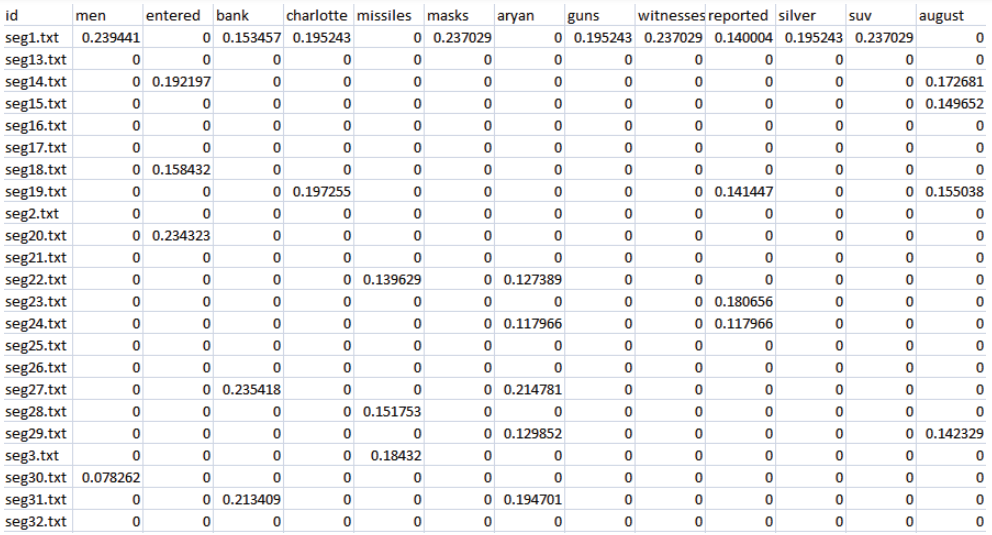
\includegraphics[width=0.8\textwidth]{1.png}
        \caption{Minh họa của các vector của các thuật ngữ trong nhiều tài liệu, bao gồm giá trị tf-idf.}
        \label{fig:1}
    \end{figure}

    Mã giả ở thuật toán \ref{alg:COMPUTE-TFIDF} tính toán các vector tf-idf cho từng tài liệu trong bộ tài liệu được cho trước.
    Thủ tục này dùng hàm COUNT-TERMS ở thuật toán \ref{alg:COUNT-TERMS}.
    Phần đầu tiên lặp qua tất cả các tài liệu, tính toán và lưu trữ tần suất của từng thuật ngữ và tần suất của từng tài liệu tương ứng với thuật ngữ.
    Phần thứ hai tính toán vecotr tf-idf cho từng tài liệu và lưu trong một bảng.

    \begin{algorithm}[h!]
        \DontPrintSemicolon
        $termFrequencies \gets \emptyset$\; \tcp{Tra cứu bảng đếm số lần thuật ngữ/từ xuất hiện cho tên tài liệu}
        $documentFrequencies \gets  \emptyset$\; \tcp*{Đếm số tài liệu mà trong đó một thuật ngữ/từ nhất định xuất hiện}
        $uniqueTerms \gets \emptyset$\; \tcp*{Danh sách các thuật ngữ/từ riêng biệt}
        \ForEach{$document$ $d$ \textbf{in} $documents$}{
            $docName \gets NAME(d)$\; \tcp{Trích xuất tên của tài liệu}
            $tokenStream \gets TOKENIZE(d)$\; \tcp{Tạo luồng token của tài liệu}
            $terms \gets COUNT-TERMS(tokenStream)$\; \tcp{Đếm tần suất của các thuật ngữ/từ}
            $termFrequencies \lbrack docName \rbrack \gets terms$\; \tcp{Lưu trữ tần suất các thuật ngữ/từ tương ứng với từng tài liệu}
            \ForEach{$term$ $t$ \textbf{in} $KEYS(terms$)}{
                \If{$t$ \textbf{not in} $documentFrequencies$} {
                    $documentFrequencies \lbrack t \rbrack \gets 1$\;
                } 
                \Else {
                    $documentFrequencies \lbrack t \rbrack \gets documentFrequencies \lbrack t \rbrack + 1$\;
                }
                $uniqueTerms \gets uniqueTerms \cup t$\;
            }
        }
        $tfIdfVectorTable \gets \emptyset$\; \tcp{Tra cứu vector tf-idf cho tên tài liệu}
        $n \gets LENGTH(documents)$\;
        \ForEach{$document$ $name$ $docName$ \textbf{in} $KEYS(termFrequencies)$}{
            $tfIdfVector \gets $ \text{zeroes array of length} $LENGTH(uniqueTerms)$\;
            $terms \gets termFrequencies \lbrack docName \rbrack$\;
            \ForEach{$term$ $t$ \textbf{in} $KEYS(terms)$}{
                $tf \gets terms \lbrack t \rbrack$\;
                $df \gets documentFrequencies \lbrack t \rbrack$\;
                $tfIdf \gets tf \times \log \Big( \dfrac{n}{df} \Big)$\;
                $tfIdfVector \lbrack \text{chỉ số của } t \text{ trong } uniqueTerms \rbrack \gets tfIdf$\;
            }
            $tfIdfVectorTable \lbrack docName \rbrack \gets tfIdfVector$\;
        }
        \Return{$tfIdfVectorTable$}\;
        \caption{COMPUTE-TFIDF(documents)}
        \label{alg:COMPUTE-TFIDF}
    \end{algorithm}

    \subsection{Định luật Zipf}

    Phân phối chuẩn và phân phối đều là các phân phối ta quen thuộc nhất.
    Phân phối hàm mũ ngày nay rất phổ biến với kích thước dữ liệu lớn, phản ánh hiện tượng mở rộng dữ liệu.
    Nhà kinh tế học Vilfredo Pareto tuyên bố rằng doanh thu của một công ty tỷ lệ nghịch với thứ hạng của công ty này, chính là tuân theo phân phối mũ kinh điển,
    dẫn đến quy tắc 80 - 20, trong đó 20\% dân số nắm giữ 80\% tài sản.

    \begin{figure}[h!]
        \centering
        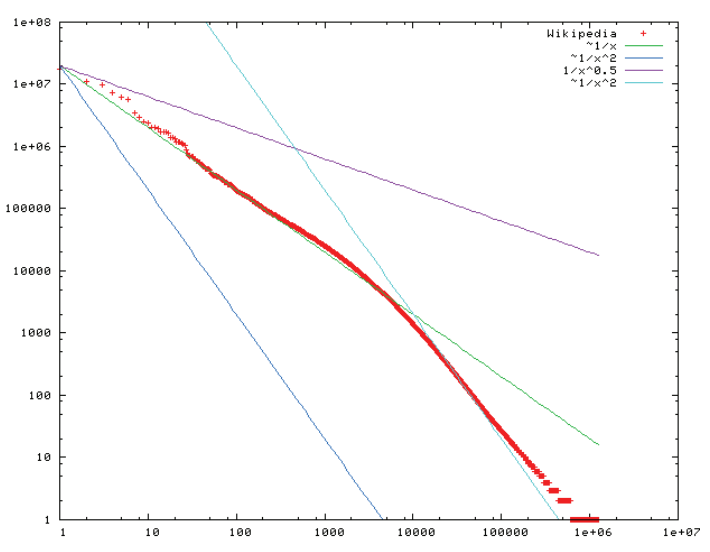
\includegraphics[width=0.8\textwidth]{2.png}
        \caption{Phân phối của các thuật ngữ trong Wikipedia, một ví dụ về luật Zipf.
        Phân phối của các thuật ngữ nằm trên trục y, và thứ hạng tần suất nằm trên trục x.}
        \label{fig:2}
    \end{figure}

    Nhà ngôn ngữ học George Kingsley Zipf tuyên bố rằng phân phối của các từ trong corpora tuân theo phân phối mũ được gọi là phân phối Zipf.
    Định luật Zipf \cite{490} phát biểu rằng trong một tài liệu ngôn ngữ tự nhiên điển hình, tần suất của một từ tỷ lệ nghịch với thứ hạng của nó trong bảng tần suất.
    Vẽ đồ thị đường cong Zipf trên thang đo log - log ta thu được một đường thẳng có hệ số góc -1 (hình \ref{fig:2}).

    Ý nghĩa của định luật Zipf là một lượng nhỏ các từ miêu tả hầu hết các khái niệm chính trong các tài liệu nhỏ.
    Có rất nhiều ví dụ về tóm tắt văn bản cho phép mô tả đầy đủ chỉ bằng một vài từ.

    \subsection{Các nhiệm vụ sử dụng mô hình không gian vector}

    Mô hình không gian vector, khi đi cùng với một độ đo khoảng cách cho phép ta thực hiện nhiều tác vụ hữu ích.
    Ta có thể sử dụng tf-idf và mô hình không gian vector để nhận diện các tài liệu cần được quan tâm đặc biệt.
    Ví dụ, mô hình không gian vector, với việc sử dụng một số độ đo khoảng cách, sẽ cho phép ta trả lời câu hỏi tài liệu nào giống với một tài liệu cụ thể cho trước,
    tài liệu nào có liên quan đến một tập các tài liệu hoặc tài liệu nào phù hợp nhất cho một truy vấn tìm kiếm cho trước,
    bằng cách tìm tất cả các tài liệu mà các vector thuật ngữ là gần nhất với tài liệu đã cho, vector trung bình trên một tập các tài liệu hoặc vector của một truy vấn tìm kiếm.

    Một nhiệm vụ gián tiếp khác là làm thế nào để giúp người dùng hiểu được ý nghĩa của toàn bộ corpus.
    Người dùng có thể đang tìm kiếm các mẫu hoặc các cấu trúc, ví dụ các chủ đề chính của tài liệu, các cụm và phân phối của các chủ đề xuyên suốt tập tài liệu.
    Điều này thường liên quan đến việc trực quan hóa corpus trong bố cục hai chiều hoặc hiển thị cho người dùng một biểu đồ kết nối giữa các tài liệu hoặc thực thể để điều hướng.
    Quá trình trực quan hóa ánh xạ đến trực quan hóa tài liệu: ta thu thập dữ liệu (tập văn bản),
    biến đổi các tà liệu này thành các vector, sau đó thực thi các thuật toán dựa trên các nhiệm vụ đang được quan tâm (đo độ tương tự, tìm kiếm, phân cụm) và thực hiện trực quan hóa.

    \begin{figure}[h!]
        \centering
        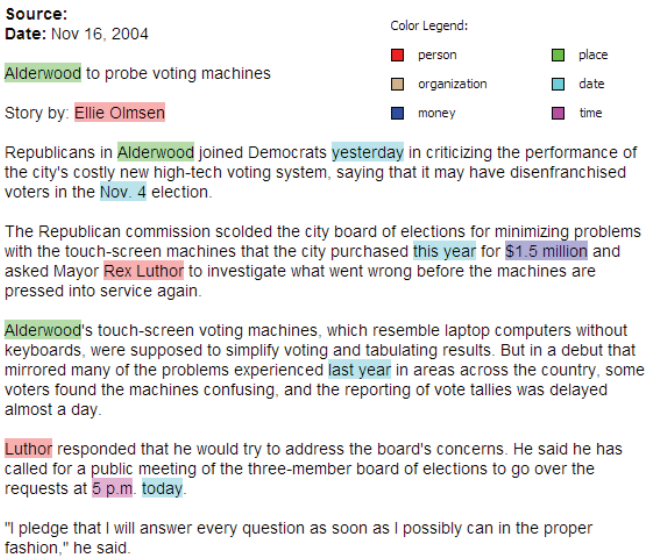
\includegraphics[width=0.8\textwidth]{3.png}
        \caption{Chế độ xem mà các thực thể có tên được tô sáng, các màu tô sáng tương ứng theo loại thực thể}
        \label{fig:3}
    \end{figure}

    \section{Trực quan hóa tài liệu đơn}

    Ở mục này ta sẽ trình bày một số phương pháp trực quan hóa dữ liệu của tài liệu văn bản đơn được lấy từ tập dữ liệu VAST Contest 2007.

    \begin{figure}[h!]
        \centering
        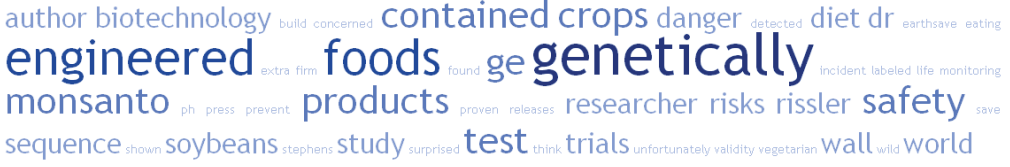
\includegraphics[width=0.8\textwidth]{4.png}
        \caption{Trực quan hóa đám mây thẻ được tạo bởi dịch vụ miễn phí tagCrowd.com \cite{396}.
        Cỡ chữ và độ tối tỷ lệ thuận với tuần suất xuất hiện của từ trong tài liệu}
        \label{fig:4}
    \end{figure}

    \subsection{Đám mây từ}

    Đám mây từ (hình \ref{fig:4}), còn được gọi là đám mây văn bản hoặc đám mây thẻ, là bố của các các token mà được tô màu và định cỡ hiển thị theo tần suất xuất hiện của chúng trong một tài liệu.
    Các đám mây văn bản và các biến thể của chúng, chẳng hạn như Wordle (hình \ref{fig:5}) là những vi dụ về sử quan quá chỉ sử dụng các vector tần suất của các thuật ngữ và một số thuật toán bố cục để tạo trực quan hóa.


    \begin{figure}[h!]
        \centering
        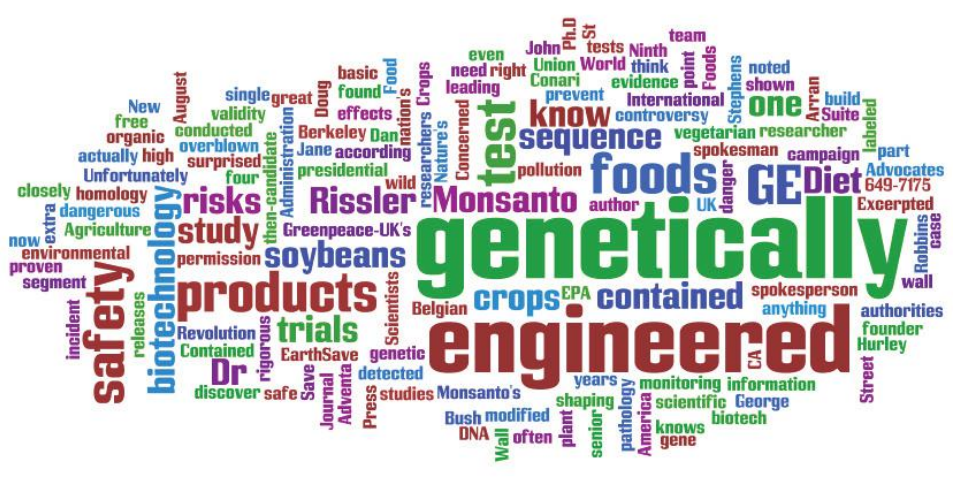
\includegraphics[width=0.8\textwidth]{5.png}
        \caption{Một Wordle được tạo bởi dịch vụ miễn phí wordle.net \cite{118}.
        Kích thước của các từ tương ứng với tần suất của từ trong tài liệu}
        \label{fig:5}
    \end{figure}

    \subsection{WordTree}

    Trực quan hóa WordTree \cite{450} là một biểu diễn trực quan của cả tần số thuật ngữ cũng như ngữ cảnh của thuật ngữ (hình \ref{fig:6}).
    Kích thước được sử dụng để đại diện cho thuật ngữ hoặc tần suất của cụm từ.
    Gốc của cây là một từ hoặc cụm từ do người dùng chỉ định và các nhánh biểu diễn các ngữ cảnh khác nhau mà từ hoặc cụm từ được sử dụng trong tài liệu.


    \begin{figure}[h!]
        \centering
        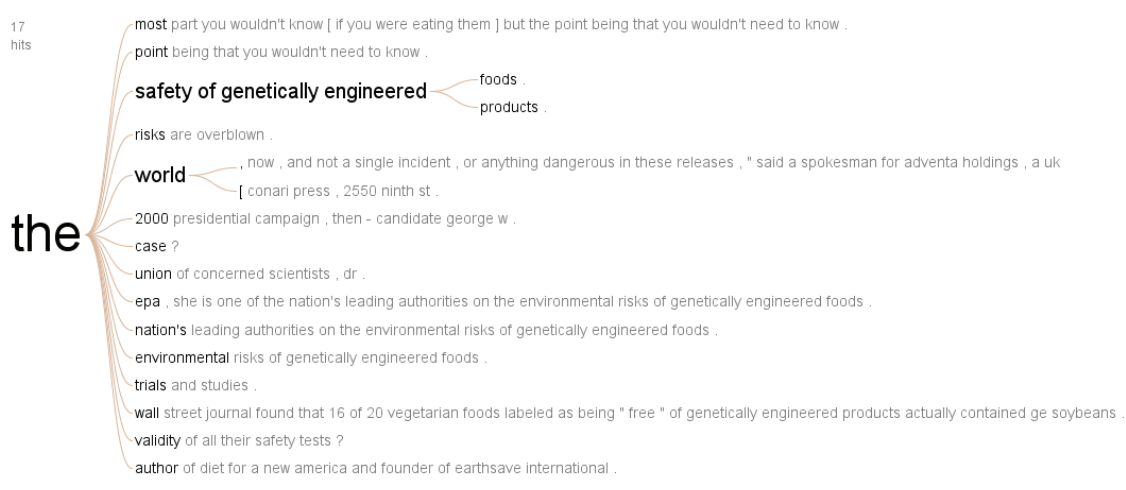
\includegraphics[width=0.8\textwidth]{6.png}
        \caption{Hình ảnh WordTree được tạo bởi dịch vụ miễn phí ManyEyes \cite{196}.
        Các nhánh của cây đại diện cho các ngữ cảnh khác nhau theo sau một từ gốc hoặc cụm từ gốc trong tài liệu}
        \label{fig:6}
    \end{figure}


    \subsection{TextArc}

    Ta có thể mở rộng biểu diễn của phân phối từ bằng cách hiển thị kết nối.
    Có nhiều cách để tính toán kết nối giữa các từ.
    TextArc \cite{312} là một biểu diễn trực quan về các thuật ngữ liên quan đến dòng văn bản mà nó xuất hiện (hình \ref{fig:7}).
    Mỗi từ trong văn bản được vẽ theo thứ tự xung quan một elip dưới dạng các dòng nhỏ với độ lệch nhẹ ở đầu.
    Cũng như trong đám mấy văn bản, các từ với tần suất cao hơn được vẽ lớn hơn và sáng hơn.
    Các từ có tần suất cao hơn được vẽ bên trong elip, kéo bởi các lần xuất hiện của nó trên hình tròn (tương tự với RadViz).
    Người dùng có thể ấn vào các chữ ẩn bên dưới bằng cách thăm dò và tạo hiệu ứng "đọc" văn bản bằng cach trực quan hóa luồn văn bản thông qua các thuật ngữ được kết nối có liên quan.

    \begin{figure}[h!]
        \centering
        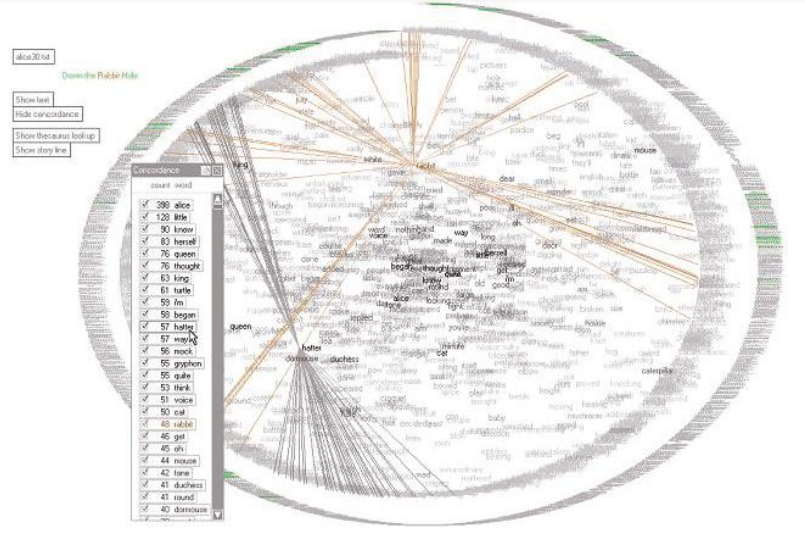
\includegraphics[width=0.9\textwidth]{7.png}
        \caption{Một hình ảnh TextArc được tạo ra sử dụng truyện "Alice in Wonderland".
        Các từ xuất hiện trong toàn bộ các phần trong tài liệu được đặt ở giữa TextArc, trong khi các từ chỉ xuất hiện trong vài phần cụ thể được đặt gần viền hơn.}
        \label{fig:7}
    \end{figure}

    \subsection{Sơ đồ vòng cung (Arc Diagrams)}

    Sơ đồ vòng cung là trực quan hóa tập trung vào việc hiển thị sự lặp lại trong văn bản.
    Các dãy con lặp đi lặp lại được xác định và được nối với nhau bằng các cung nửa hình tròn.
    Độ dày của các cung biểu diễn độ dài của các dãy con và độ cao của các cung biểu diễn khoảng cách giữa các dãy con.
    Hình \ref{fig:8} hiển thị "Bach’s Minuet in G Major", trực quan hóa mô hình cổ điển của điệu nhảy Minuet.
    Nó bao gồm hai phần, mỗi phần gồm một bước dài được đi hai lần.
    Các phần có liên quan không mật thiết, được thể hiện bởi các vòng cung mỏng kết nối hai phần chính.
    Sự trùng lặp của hai cung chính cho thấy đoạn cuối của phần đầu giống với đoạn đầu của phần thứ hai

    \begin{figure}[h!]
        \centering
        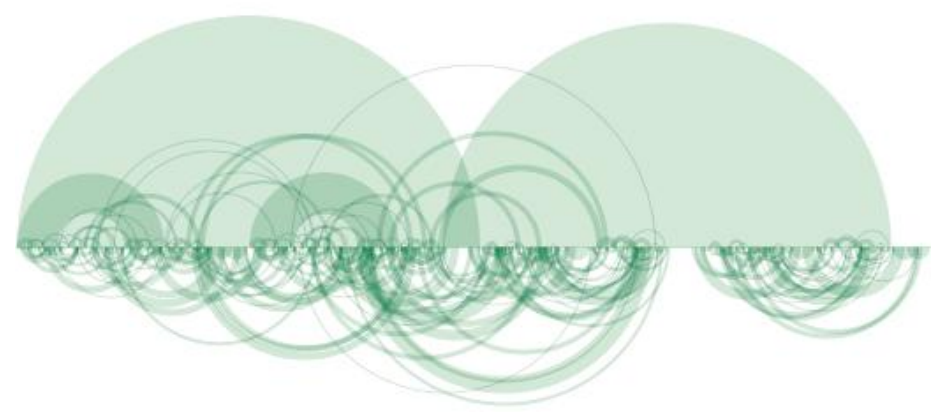
\includegraphics[width=0.9\textwidth]{8.png}
        \caption{Một hình ảnh sơ đồ vòng cung của "Bach’s Minuet in G Major".
        Các dãy lặp lại được kết nối bằng một đường cong nửa hình tròn. \cite{451}}
        \label{fig:8}
    \end{figure}

    \subsection{Dấu ấn văn học (Literature Fingerpriting)}


    Dấu ấn văn học là một phương pháp trực quan hóa các đặc trưng được sử dụng để thể hiện các đặc tính của văn bản \cite{222}.
    Thay vì chỉ tính toán một giá trị đặc trưng hoặc một vector cho toàn bộ văn bản (đây là điều hay thường được thực hiện), ta tính toán một dãy các giá trị đặc trưng từng văn bản và hiển thị chúng cho người dùng dưới dạng dấu ấn đặc trưng của tài liệu.
    Điều này cho phép người dùng hiểu tài liệu và phân tích sự phát triển của các giá trị trên toàn văn bản.
    Hơn nữa, thông tin cấu trúc của tài liệu được dùng để trực quan hóa tài liệu trên nhiều cấp độ khác nhau của độ phân giải.
    Dấu ấn văn học được áp dụng cho bài toán xác nhận quyền tác giả để thể hiện khả năng phân biệt của các độ đo tiêu chuẩn được giả định để nắm bắt được phong cách sáng tác của một tác giả (hình \ref{fig:9}).

    \begin{figure}[h!]
        \centering
        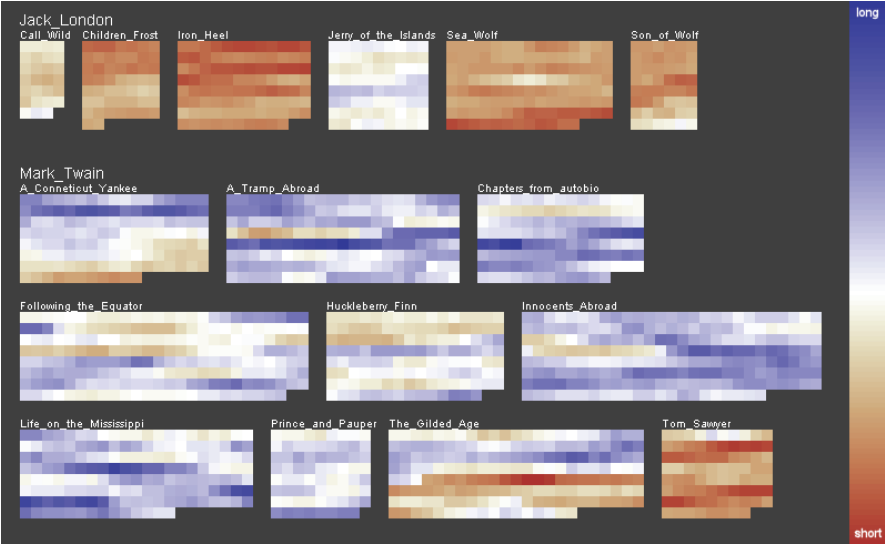
\includegraphics[width=0.9\textwidth]{9.png}
        \caption{Kỹ thuật lấy dấu ấn văn học. Dấu ấn văn học được sử dụng để phân tích nhiều độ đo văn bản để phân biệt tác giả của tài liệu.
        Từng điểm ảnh biểu diễn một khối văn bản, các điểm ảnh được ghép lại thành các cuốn sách.
        Màu các điểm ảnh được ảnh xạ từ các giá trị đặc trưng, trong trường hợp này là độ dài trung bình của câu.
        Nếu một độ đo có khả năng phân biệt giữa hai tác giả, các sách ở hàng đầu tiên được viết bởi Jack London và các sách còn lại được viết bởi Mark Twain. \cite{222}}
        \label{fig:9}
    \end{figure}

    \section{Trực quan hóa tập tài liệu}

    Trong hầu hết các trường hợp trực quan hóa tập tài liệu, mục tiêu đặt ra là đặt các tài liệu tương tự nhau ở gần nhau và các tài liệu khác nhau cách xa nhau.
    Đây là bài toán đối kháng và thường có độ phức tạp $O(n^2)$.
    Ta tính toán sự giống nhau giữa tất cả từng cặp tài liệu và xác định bố cục.
    Cách tiếp cẩn phổ biến là bố cục lò xo đồ thị, chia tỷ lệ đa chiều, phân cụm (k-means, phân cấp, tối đa hóa kỳ vọng (EM), vector hỗ trợ) và bản đồ tự tổ chức.
    Ta trình bày một vài kỹ thuật trực quan hóa tập tài liệu như bản đồ tự tổ chức, bản đồ cụm và các hình nền chủ đề.

    \subsection{Bản đồ tự tổ chức}

    Bản đồ tự tổ chức (SOM) \cite{248} là một thuật toán học không giám sát bằng cách sử dụng một tập các nút thường là 2 chiều, vị trí mà tài liệu sẽ được đặt.
    Từng nút có một vector tưng ứng với cùng số chiều với vector đầu vào (các vector tài liệu) được sử dụng để huấn luyện bản đồ.
    Ta khởi tạo các nút của SOM, thường có các trọng số ngẫu nhiên.
    Ta chọn một ector ngẫu nhiên từ các vector đầu vào và tính toán khoảng cách của nó đến từng mỗi nút khác.
    Ta điều chỉnh trọng số của các nút gần hất (trong một bán kính cụ thể), làm cho mỗi nút gần hơn tới vector đầu vào,
    với trọng số đầu vào cao hơn tương ứng với nút được chọn gần nhất.
    Khi ta lặp qua các vector đầu vào, bán kính sẽ nhỏ hơn.
    Một ví dụ sử dụng bản đồ tự tổ chức cho dữ liệu văn bản được minh họa trong hình \ref{fig:10} \cite{454},
    hiển thị một triệu tài liệu được thu thập từ 83 nhóm tin tức.
    

    \subsection{Hình nền chủ đề}

    Hình nền chủ đề là bản tóm tắt của corpora sử dụng phong cảnh 3 chiều trừu tượng, trong đó chiều cao và màu sắc được sử dụng để biểu diễn mật độ của các tài liệu tương tự giống nhau.
    Một ví dụ được minh họa trong hình \ref{fig:11} từ Pacific Northwest National Labs \cite{407} đại diện cho các bài báo được trực quan hóa dưới dạng hình nền chủ đề.
    Các ngọn núi ao hơn biểu thị tần suất chủ đề cao hơn trong kho tài liệu (chiều cao tỷ lệ thuận với số lượng tài liệu liên quan đến chủ đề).

    \begin{figure}[h!]
        \centering
        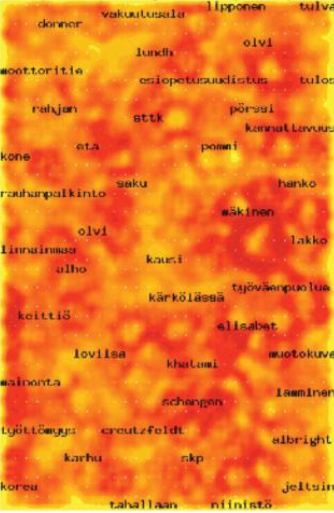
\includegraphics[width=0.5\textwidth]{10.png}
        \caption{Bố cục bản đồ tự tổ chức của mục bản tin Phần Lan.
        Các nhãn hiển thị các khu vực chủ đề và màu sắc biểu thị số lượng các tài liệu tương ứng với chủ đề, với các vùng càng sáng chứa nhiều tài liệu hơn \cite{454}.}
        \label{fig:10}
    \end{figure}

    \begin{figure}[h!]
        \centering
        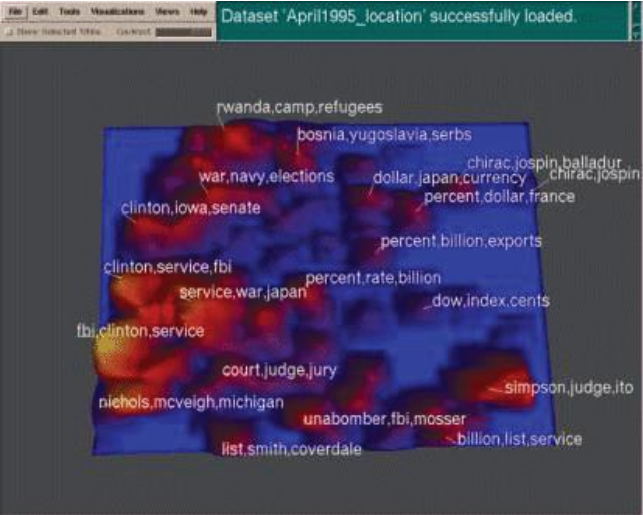
\includegraphics[width=0.6\textwidth]{11.png}
        \caption{Một hình nền chủ đề từ PNNL sử dụng chiều cao để biểu diễn tần suất xuất hiện của các chủ đề trong các bài báo. (Hình ảnh được in từ \cite{407} với sự cấp phép của  Springer Science and Business Media).}
        \label{fig:11}
    \end{figure}

    \subsection{Thẻ tài liệu}

    Thẻ tài liệu là một cách trực quan hóa thu gọn (hình \ref{fig:12}) biểu diễn ngữ nghĩa chính của tài liệu dưới dạng hỗn hợp hình ảnh và các thuật ngữ chính quan trọng, tương tự như thẻ trong trò chơi át chủ bài \cite{400}.
    Các thuật ngữ chính được trích xuất bằng cách sử dụng một cách tiếp cận khai phá văn bản nâng cao dựa trên trích xuất tự động của cấu trúc tài liệu.
    Các hình ảnh và chú thích được trích xuất sử dụng heuristic đồ họa và các thích được sử dụng cho các trọng số ảnh bán ngữ nghĩa.
    Hơn nữa, phân phối màu của ảnh được dùng để phân loại hình ảnh vào các lớp (lớp 1: ảnh chụp/ảnh kết xuất, lớp 2: sơ đồ/bản phác thảo/đồ thị, lớp 3: bảng) và hiển thị ít nhất một đại diện từ mỗi lớp không rỗng.

    \begin{figure}[h!]
        \centering
        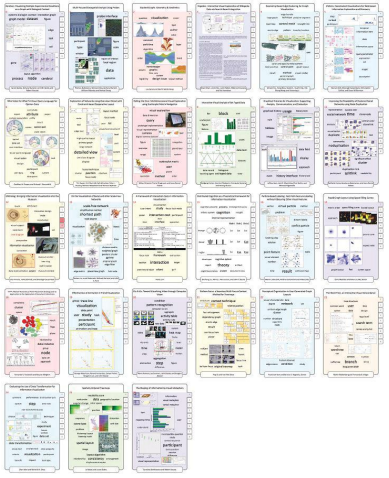
\includegraphics[width=0.95\textwidth]{12.png}
        \caption{Kho tài liệu của hội nghị IEEE InfoVis 2008 được biểu diễn bằng một ma trận các thẻ tài liệu.
        Tuần suất của các thuật ngữ trên từng trang được hiển thị ở bên tay phải của thẻ lại liệu (màu càng đỏ thể hiện tần số càng cao, ta có thể thấy ở tài liệu thứ nhất ở hàng thứ 3) \cite{400}.}
        \label{fig:12}
    \end{figure}

    \section{Các kỹ thuật trực quan hóa văn bản mở rộng}

    Mục này ta sẽ tìm hiểu nhiều kỹ thuật trực quan hóa văn bản liên quan đến metadata hay nói cách khác là vượt qua các cách trực quan hóa dựa trên vector thuật ngữ.

    \subsection{Trực quan hóa phần mềm}

    Eick và các cộng sự đã phát triển một công cụ trực quan hóa có tên là SeeSoft \cite{108} giúp trực quan hóa số liệu thống kê cho từng dòng code (tuổi và số thay đổi, lập trình viên, ngày tháng).
    Hình \ref{fig:13}, từng cột biểu diễn một file mã nguồn với chiều cao biểu thị kích thước của file.
    Nếu như file dài hơn màn hình, nó sẽ tiếp tục được biểu diễn ở cột tiếp theo.
    Trong biểu diễn của SeeSoft, từng hàng biểu diễn một dòng code.
    Vì số lượng dòng quá lớn cho một hàng, nên mỗi dòng được biểu diễn bởi một điểm ảnh trong hàng ngang.
    Điều này làm tăng số dòng có thể được hiển thị.
    Màu sắc được sử dụng để biểu thị số lần được gọi.
    Dòng càng màu đỏ thì dòng này càng được gọi nhiều, được gọi là điểm nóng (key hotspot).
    Một dòng màu xanh thể hiện ít được gọi hơn.
    Màu sắc có thể được sử dụng để biểu diễn các tham số khác, ví dụ như thời gian sửa đổi lần cuối hoặc số lần sửa đổi.
    Đối với màn hình có độ phân giải 1000x1000, SeeSoft có khả năng hiển thị lên tới 50000 dòng code.
    Hình ảnh bao gồm 53 file với 15255 dòng code. 
    File được lựa chọn là file1.c, một khối code được phóng to của dòng code 408.

    \begin{figure}[h!]
        \centering
        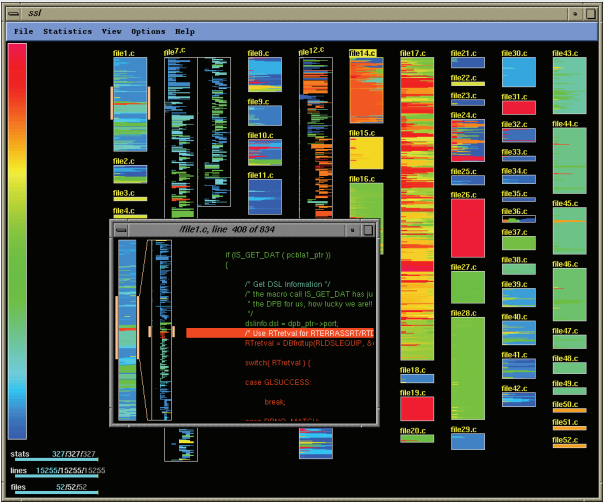
\includegraphics[width=0.95\textwidth]{13.png}
        \caption{Trực quan hóa sử dụng phần mềm SeeSoft. Các hình chữ nhật biểu diễn các file mã nguồn.
        Kích thước của các hình chữ nhật trong từng cột tương ứng với độ dài của file mã nguồn, và màu sắc của từng dòng biểu diễn các tham số liên quan đến việc sửa đổi \cite{108}.}
        \label{fig:13}
    \end{figure}

    \subsection{Trực quan hóa kết quả truy vấn}

    Marti Hearst đã phát triển một công cụ trực quan hóa kết quả truy vấn đơn giản về cơ bản tương tự như của \cite{232} được gọi là TileBars \cite{178},
    hiển thị một số thống kê liên quan đến thuật ngữ, bao gồm tần suất và phân phối của thuật ngữ, độ dài của tài liệu, xếp hạng dựa trên thuật ngữ và sức mạnh của xếp hạng.
    Mỗi tài liệu của tập kết quả được biểu diễn bằng một hình chữ nhật, trong đó chiều rộng biểu thị chiều dài tương dối của tài liệu và các ô vuông xếp chồng tương ứng với các đoạn văn bản (hình \ref{fig:14}).
    Mỗi hàng của ngắn xếp đại diện cho tập các thuật ngữ truy vấn và mức độ tối của hình vuông thể hiện tần suất của các thuật ngữ trong số các thuật ngữ tương ứng.
    Tiêu đề và những từ mở đầu từ tài liệu xuất hiện bên cạnh TileBar.
    Mỗi hình chữ nhật lớn biểu diễn một văn bản, mỗi hình vuông trong tài liệu biểu diễn một đoạn văn bản.
    Ô càng tối thì tập hợp thuật ngữ truy vấn càng có tần suất lớn.
    Điều này tạo ra một biểu diễn thu gọn và cung cấp các phản hồi về cấu trúc tài liệu phản ánh độ dài tương đối của tài liệu,
    tần suất của thuật ngữ truy vấn và phân phối của các thuật ngữ truy vấn.

    \begin{figure}[h!]
        \centering
        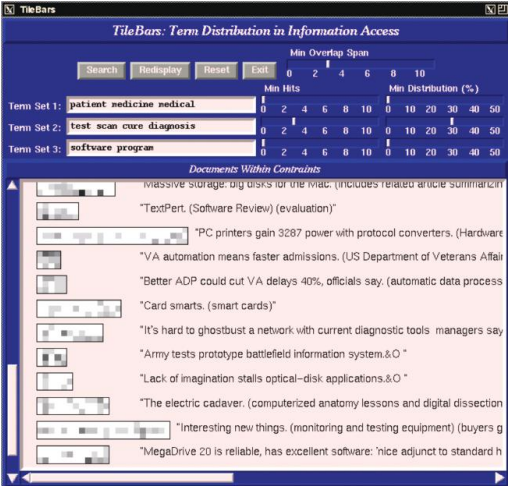
\includegraphics[width=0.95\textwidth]{14.png}
        \caption{Trực quan hóa kết quả truy vấn TileBars.
        Mỗi hình chữ nhật lớn biểu thị một tài liệu, mỗi hình vuông bên trong tài liệu biển diễn một đoạn văn bản.
        Ô càng tối thì tập hợp thuật ngữ truy vấn có tần suất càng lớn \cite{178}.}
        \label{fig:14}
    \end{figure}

    \subsection{Trực quan hóa tập tài liệu theo thời gian}

    ThemeRiver \cite{173} còn được gọi là biểu đồ luồng, là một kỹ thuật trực quan hóa các thay đổi chủ đề theo thời gian trong tập tài liệu (hình \ref{fig:15}).
    Hình ảnh trực quan này giả định rằng dữ liệu đầu vào tiến triển theo thời gian.
    Các chủ đề được thể hiện trực quan dưới dạng các dải màu nằm ngang có độ dày theo chiều dọc ở một vị trí theo chiều ngang nhất định biểu diễn tần suất của tại một thời điểm cụ thể.

    \begin{figure}[h!]
        \centering
        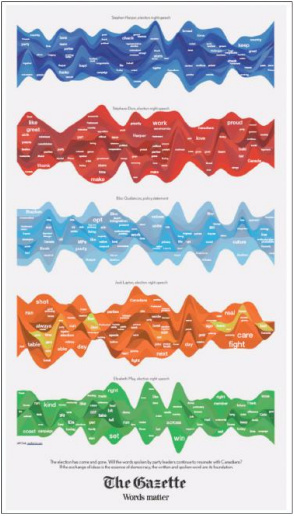
\includegraphics[width=0.5\textwidth]{15.png}
        \caption{Biểu đồ luồng (ThemeRiver) miêu tả các bài phát biểu trong đêm bầu cử của một số ứng viên khác nhau cho cuộc bầu cử ở Canada \cite{173}.}
        \label{fig:15}
    \end{figure}


    \begin{figure}[h!]
        \centering
        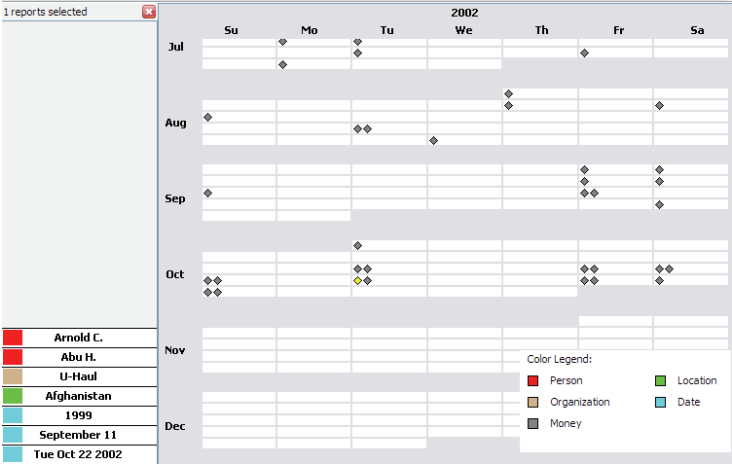
\includegraphics[width=0.9\textwidth]{16.png}
        \caption{Các bài báo được trình bày dưới dạng xem lịch Jigsaw, dựa trên các thực thể ngày được trích xuất \cite{155}.}
        \label{fig:16}
    \end{figure}


    \begin{figure}[h!]
        \centering
        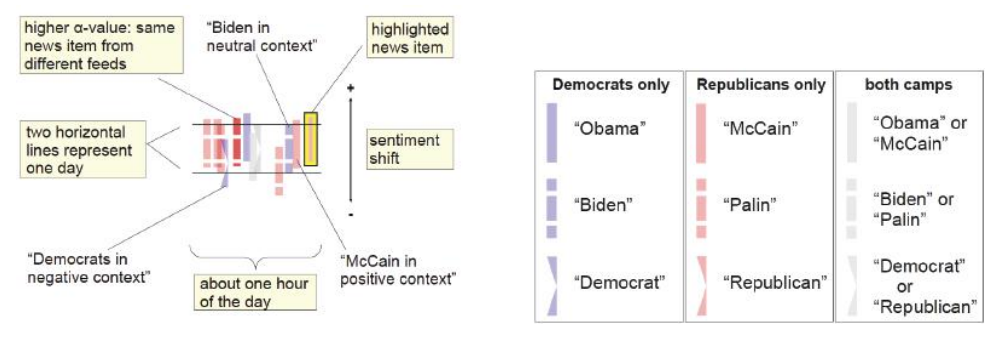
\includegraphics[width=0.9\textwidth]{17.png}
        \caption{Trực quan hóa phân tích cảm xúc \cite{440},
        Các mục tin tức được vẽ dọc theo trục thời gian.
        Hình dạng và màu sắc cho biết từng mục thuộc về danh mục nào và vị trí theo trục thẳng đứng phụ thuộc vào điểm số cảm xúc được xác định tự động của mục đó.
        Các đối tượng trực giác biểu diễn các mục tin tức được tô màu bán trong suốt để làm cho các mục chồng vào nhau dễ phân biệt hơn.}
        \label{fig:17}
    \end{figure}


    \begin{figure}[h!]
        \centering
        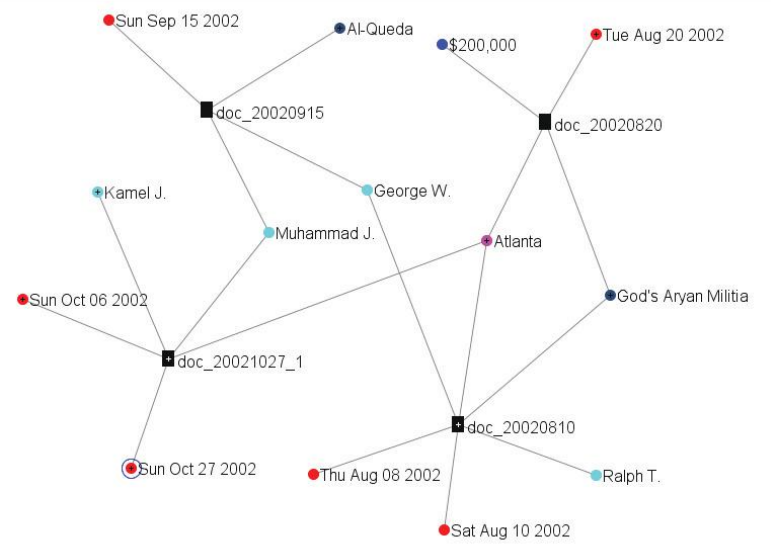
\includegraphics[width=0.9\textwidth]{18.png}
        \caption{Chế độ xem đồ thị Jigsaw, thể hiện các kết nối giữa các thực thể và tài liệu được đặt tên \cite{155}.}
        \label{fig:18}
    \end{figure}


    \begin{figure}[h!]
        \centering
        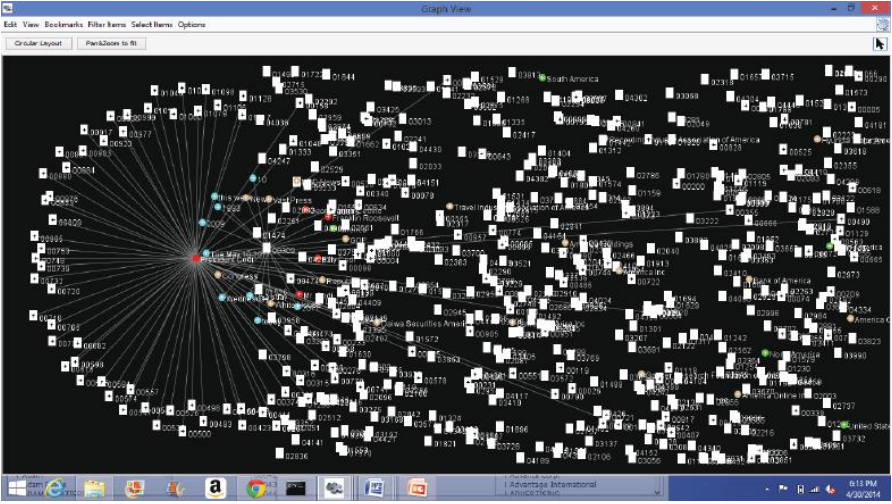
\includegraphics[width=0.9\textwidth]{19.png}
        \caption{Chế độ xem đồ thị phân cụm trong Jigsaw lọc các tài liệu có các thực thể cụ thể.
        Di chuột qua một thực thể xác định dữ liệu về tài liệu.
        Màu sắc đại diện cho giá trị tokens.}
        \label{fig:19}
    \end{figure}


    \begin{figure}[h!]
        \centering
        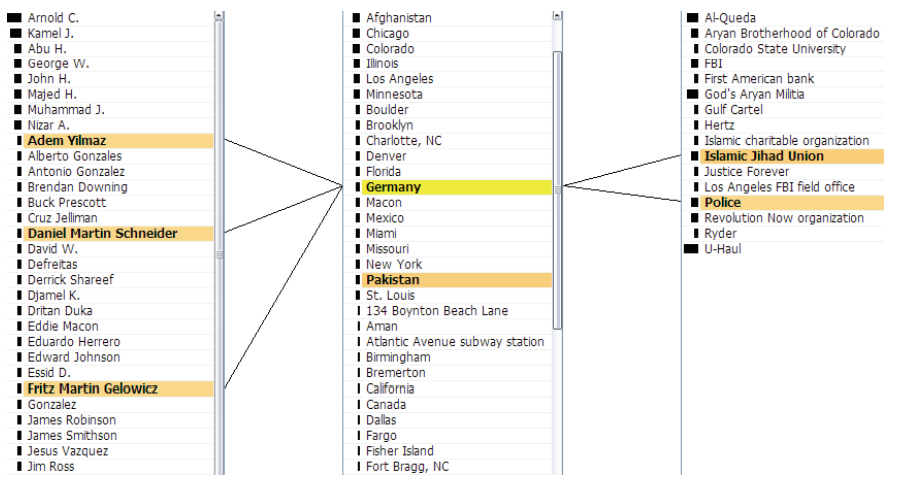
\includegraphics[width=0.9\textwidth]{20.png}
        \caption{Chế độ xem danh sách Jigsaw, hiển thị các kết nối giữa mọi người (bên trái), các địa điểm (giữa) và các tổ chức (bên phải) \cite{155}.}
        \label{fig:20}
    \end{figure}

    \newpage
    
    \printbibliography[title={TÀI LIỆU THAM KHẢO}]
\end{document}